\section{Fase 4: execução, resultados e julgamento}
\label{sec:fase4}

A coleta ocorreu de 15 a 22/11/2026, com a matriz complementar em 23/11, na versão v4.15.10.116 do SIGAA (a Fase 1 registrou a v4.15.10.115; a mudança foi registrada, como prevê o plano). Cinco estudantes participaram do teste com usuários, dois do começo e três do meio ou do fim do curso, somando 30 tentativas das seis tarefas; os participantes são identificados como P1, P2, P3, P4 e P6. As inspeções de M1, M2, M10 e M20 tiveram dois avaliadores, o primeiro deles um \textit{script} que registra as evidências e o segundo, humano, que repetiu os pontos decisivos (teclado, leitor de tela e bloqueio de \textit{pop-ups}); não houve divergência. O WAVE foi aplicado às seis páginas finais das tarefas, M13 foi executada em 24 combinações de navegador e tarefa, M14 em 12 verificações (seis páginas em 360 e 768~px) e M15 em um celular real. Todas as 16 métricas foram calculadas, e todas receberam nível.

\textbf{Desvios do plano.} Quatro desvios foram registrados e tratados: (i) o teste foi feito com cinco estudantes, um a menos que o planejado, e o grupo do começo do curso ficou com dois; (ii) nas inspeções, o primeiro avaliador foi um \textit{script} que registra evidências, e não uma pessoa, e o segundo avaliador repetiu manualmente os pontos decisivos; (iii) M14 foi verificada por emulação, e não em celular real, porque as falhas decorrem da largura e da ausência de \textit{viewport}, que a emulação reproduz (a matriz multiplataforma, Seção~\ref{sec:matriz}, confirma o resultado em 10 perfis móveis); e (iv) Edge e Safari, que exigem outro sistema operacional, foram executados em um computador com macOS por outro membro, com referência própria no Chrome. Nenhum desvio alterou as fichas, as faixas ou as regras de julgamento.

\subsection{Resultado das métricas}

A Tabela~\ref{tab:resultados} traz o valor e o nível de cada métrica, que é também o nível da sua questão (etapa 1 do julgamento), e a Fig.~\ref{fig:metricas} mostra onde cada valor caiu nas faixas fixadas na Fase 2. Das 16 questões, uma ficou Excelente (6,25\%), quatro Bom (25\%), cinco Regular (31,25\%) e seis Insatisfatório (37,5\%).

\begin{figure*}[!t]
	\centering
	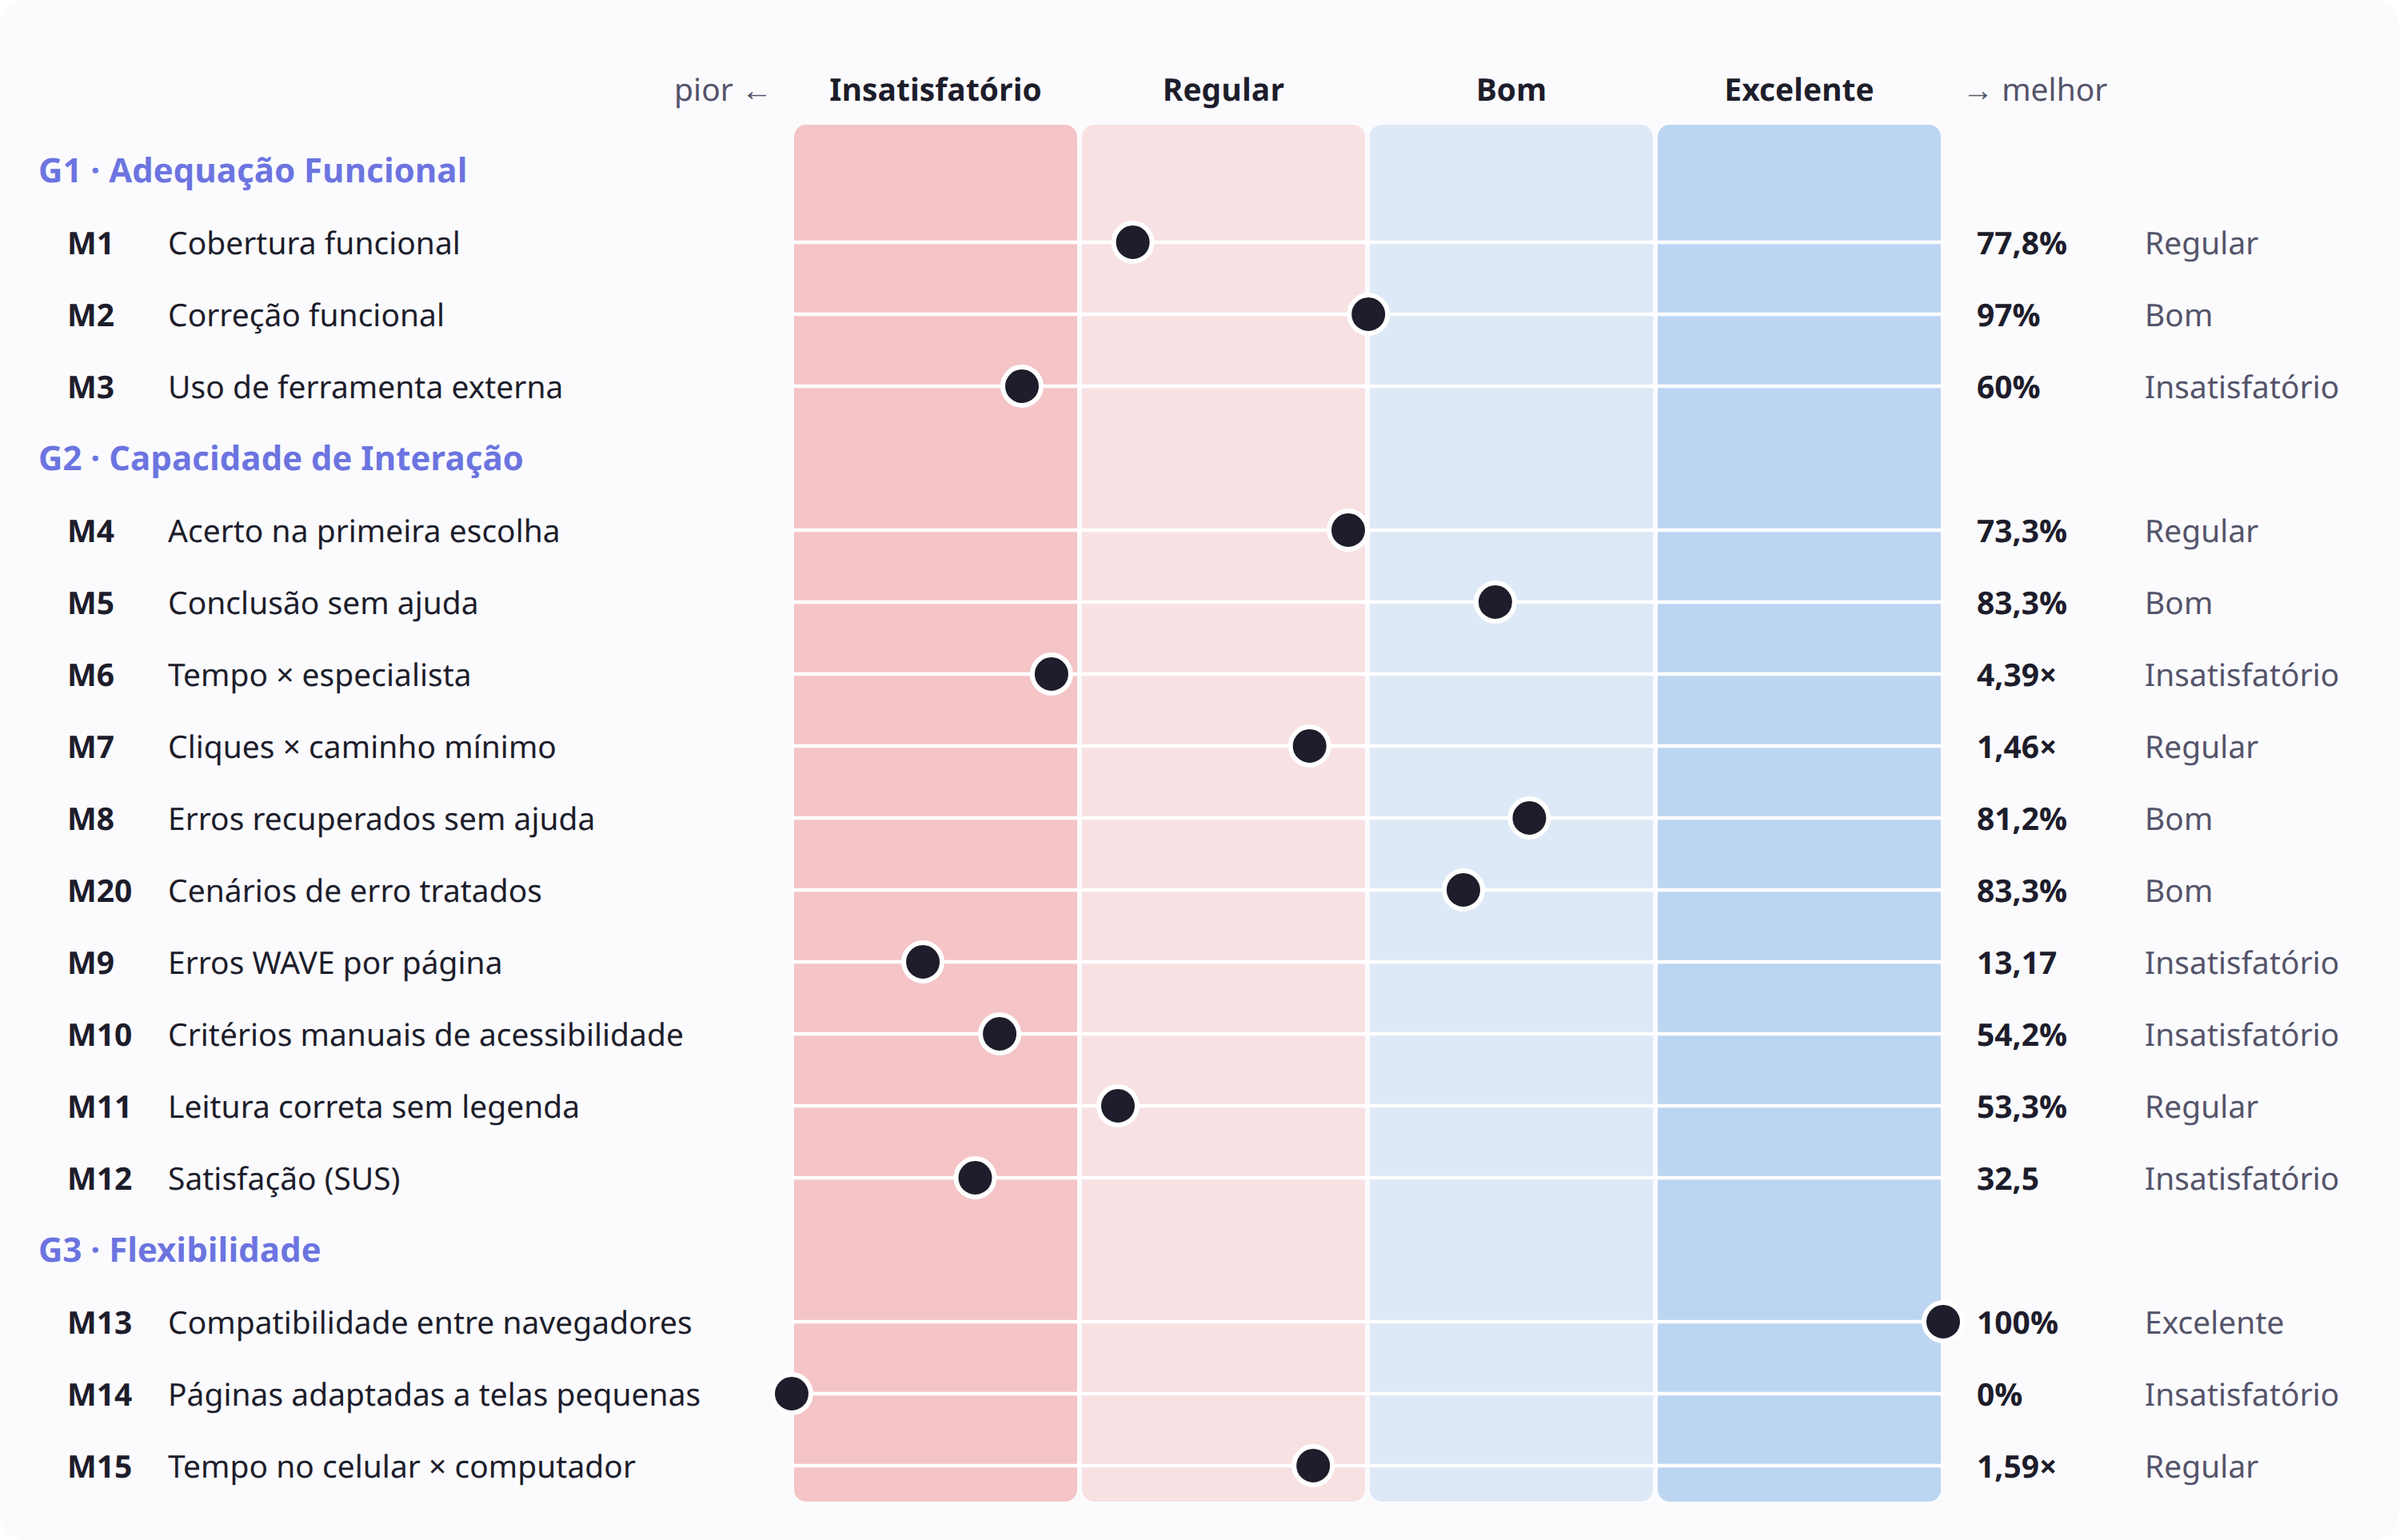
\includegraphics[width=0.8\textwidth]{figuras/metricas.png}
	\caption{Valor e nível das 16 métricas nas faixas definidas na Fase 2, por característica. As faixas têm a mesma largura; o ponto fica na posição do valor dentro da sua faixa.}
	\label{fig:metricas}
	\fonte{elaborado pela equipe a partir de \texttt{dados/consolidados/metricas.csv}.}
\end{figure*}

\begin{table}[!t]
	\caption{Valor e nível de cada métrica}
	\label{tab:resultados}
	\centering
	\footnotesize
	\setlength{\tabcolsep}{3pt}
	\begin{tabularx}{\columnwidth}{C{0.55cm} Y C{1.75cm} C{1.25cm}}
		\toprule
		\textbf{Q} & \textbf{Métrica} & \textbf{Valor} & \textbf{Nível} \\
		\midrule
		\multicolumn{4}{l}{\textit{G1 -- Adequação Funcional}} \\
		Q1 & M1 Cobertura funcional & 77,8\% (14/18) & Regular \\
		Q2 & M2 Correção funcional & 97,0\% (65/67) & Bom \\
		Q3 & M3 Uso de ferramenta externa & 60\% (3/5) & Insatisf. \\
		\midrule
		\multicolumn{4}{l}{\textit{G2 -- Capacidade de Interação}} \\
		Q4 & M4 Acerto na primeira escolha & 73,3\% (22/30) & Regular \\
		Q5 & M5 Conclusão sem ajuda & 83,3\% (25/30) & Bom \\
		Q6 & M6 Tempo relativo ao especialista & 4,39 & Insatisf. \\
		Q7 & M7 Desvio de caminho & 1,46 & Regular \\
		Q8 & M8 Recuperação de erros & 81,3\% (13/16) & Bom \\
		Q9 & M20 Cenários de erro tratados & 83,3\% (5/6) & Bom \\
		Q10 & M9 Erros WAVE por página & 13,17 (79/6) & Insatisf. \\
		Q11 & M10 Critérios manuais de acessibilidade & 54,2\% (13/24) & Insatisf. \\
		Q12 & M11 Leitura correta sem legenda & 53,3\% (8/15) & Regular \\
		Q13 & M12 Satisfação (SUS) & 32,5 & Insatisf. \\
		\midrule
		\multicolumn{4}{l}{\textit{G3 -- Flexibilidade}} \\
		Q14 & M13 Compatibilidade de navegadores & 100\% (24/24) & Excelente \\
		Q15 & M14 Páginas adaptadas & 0\% (0/12) & Insatisf. \\
		Q16 & M15 Tempo no celular & 1,59 & Regular \\
		\bottomrule
	\end{tabularx}
	\fonte{elaborado pela equipe a partir de \texttt{dados/consolidados/metricas.csv}.}
\end{table}

\textbf{Adequação Funcional.} Das 18 funções da lista de referência, 14 existem; todas as funções das tarefas T1 a T6 existem, e as quatro ausentes são de planejamento do curso (fluxo com o que já foi cursado, planejamento dos semestres, grade de horários antes da matrícula e simulação do IRA), justamente as oferecidas pelas ferramentas da comunidade. As 44 menções da tela de notas, o IRA, a MP e as cargas horárias pendentes coincidem com o histórico; as duas divergências de M2 são datas do calendário (um dia no SIGAA, dois no calendário da SAA), sem efeito em prazos do estudante. Três dos cinco participantes planejam o curso fora do SIGAA.

\textbf{Capacidade de Interação.} Os participantes concluíram sem ajuda 25 das 30 tentativas e se recuperaram sozinhos de 13 dos 16 erros, mas levaram, em média, 4,39 vezes o tempo do especialista (8,48 vezes em T4), fizeram 1,46 vez os cliques do caminho mínimo e erraram a primeira escolha de menu em 8 das 30 tentativas. Só 40\% interpretaram sem a legenda o código de horário de T2 (``24M34''). Nenhuma pontuação SUS individual alcançou o nível Regular (de 17,5 a 45,0). Na acessibilidade, o WAVE encontrou 79 erros nas seis páginas, 37 deles na Turma Virtual; na inspeção manual, o menu principal (Ensino) não recebe o foco do teclado e é anunciado pelo leitor de tela sem nome, de modo que T1, T3, T4 e T6, que começam por ele, não podem ser feitas sem mouse. O sistema tratou cinco dos seis cenários de erro; o não tratado é a sessão expirada, que leva de volta ao portal sem mensagem.

\textbf{Flexibilidade.} No computador, as seis tarefas funcionaram nos quatro navegadores do plano (Chrome, Firefox, Edge e Safari/WebKit). No celular e no tablet, nenhuma página se adapta: as páginas não declaram a \textit{viewport} (\texttt{<meta name=viewport>}) e têm \textit{layout} de 980~px, que o navegador reduz a 37\% da escala em 360~px e a 78\% em 768~px. A menor fonte efetiva fica entre 2,9 e 3,8~px em 360~px, todos os 1.063 textos ficam abaixo dos 12~px da ficha, e o item Ensino do menu vira um alvo de 22,8~$\times$~8,8~px. No celular real (Samsung Galaxy S25 Ultra, com o Chrome e a mesma rede Wi-Fi do computador), as seis tarefas levaram 110,2~s, contra 69,1~s no computador (1,59 vez), com as maiores razões nas páginas de tabelas e menus: T2 (2,03), T5 (1,96) e T6 (1,89). No questionário, os cinco participantes disseram usar o SIGAA no celular e precisar de \textit{zoom} e rolagem lateral.

\subsection{Hipóteses e julgamento}

\textbf{Hipóteses.} A Fig.~\ref{fig:hipoteses} compara o nível previsto e o obtido em cada hipótese. Foram confirmadas H1, H4, H7, H10, H12, H15 e H16 (7) e refutadas H2, H3, H5, H6, H8, H9, H11, H13 e H14 (9); nenhuma ficou inconclusiva. H5 foi refutada pelo recorte dos calouros: eles concluíram 10 das 12 tentativas (83,3\%), o mesmo que os estudantes do meio ou do fim do curso, e não menos de 65\%, como previsto; a diferença entre os grupos apareceu na satisfação (SUS médio de 22,5 contra 39,2). As refutações para pior (H2, H3, H6, H11 e H13) concentram-se no tempo, na satisfação, na acessibilidade manual e no uso de ferramentas externas: a Fase 1 tratava o SIGAA como ``usável, porém trabalhoso'', e os dados mostram que ele é mais demorado, menos satisfatório e mais dependente do mouse do que isso. As refutações para melhor (H5, H8, H9 e H14) estão na conclusão pelos calouros, na recuperação de erros, no tratamento de cenários de erro e na compatibilidade entre navegadores.

\begin{figure*}[!t]
	\centering
	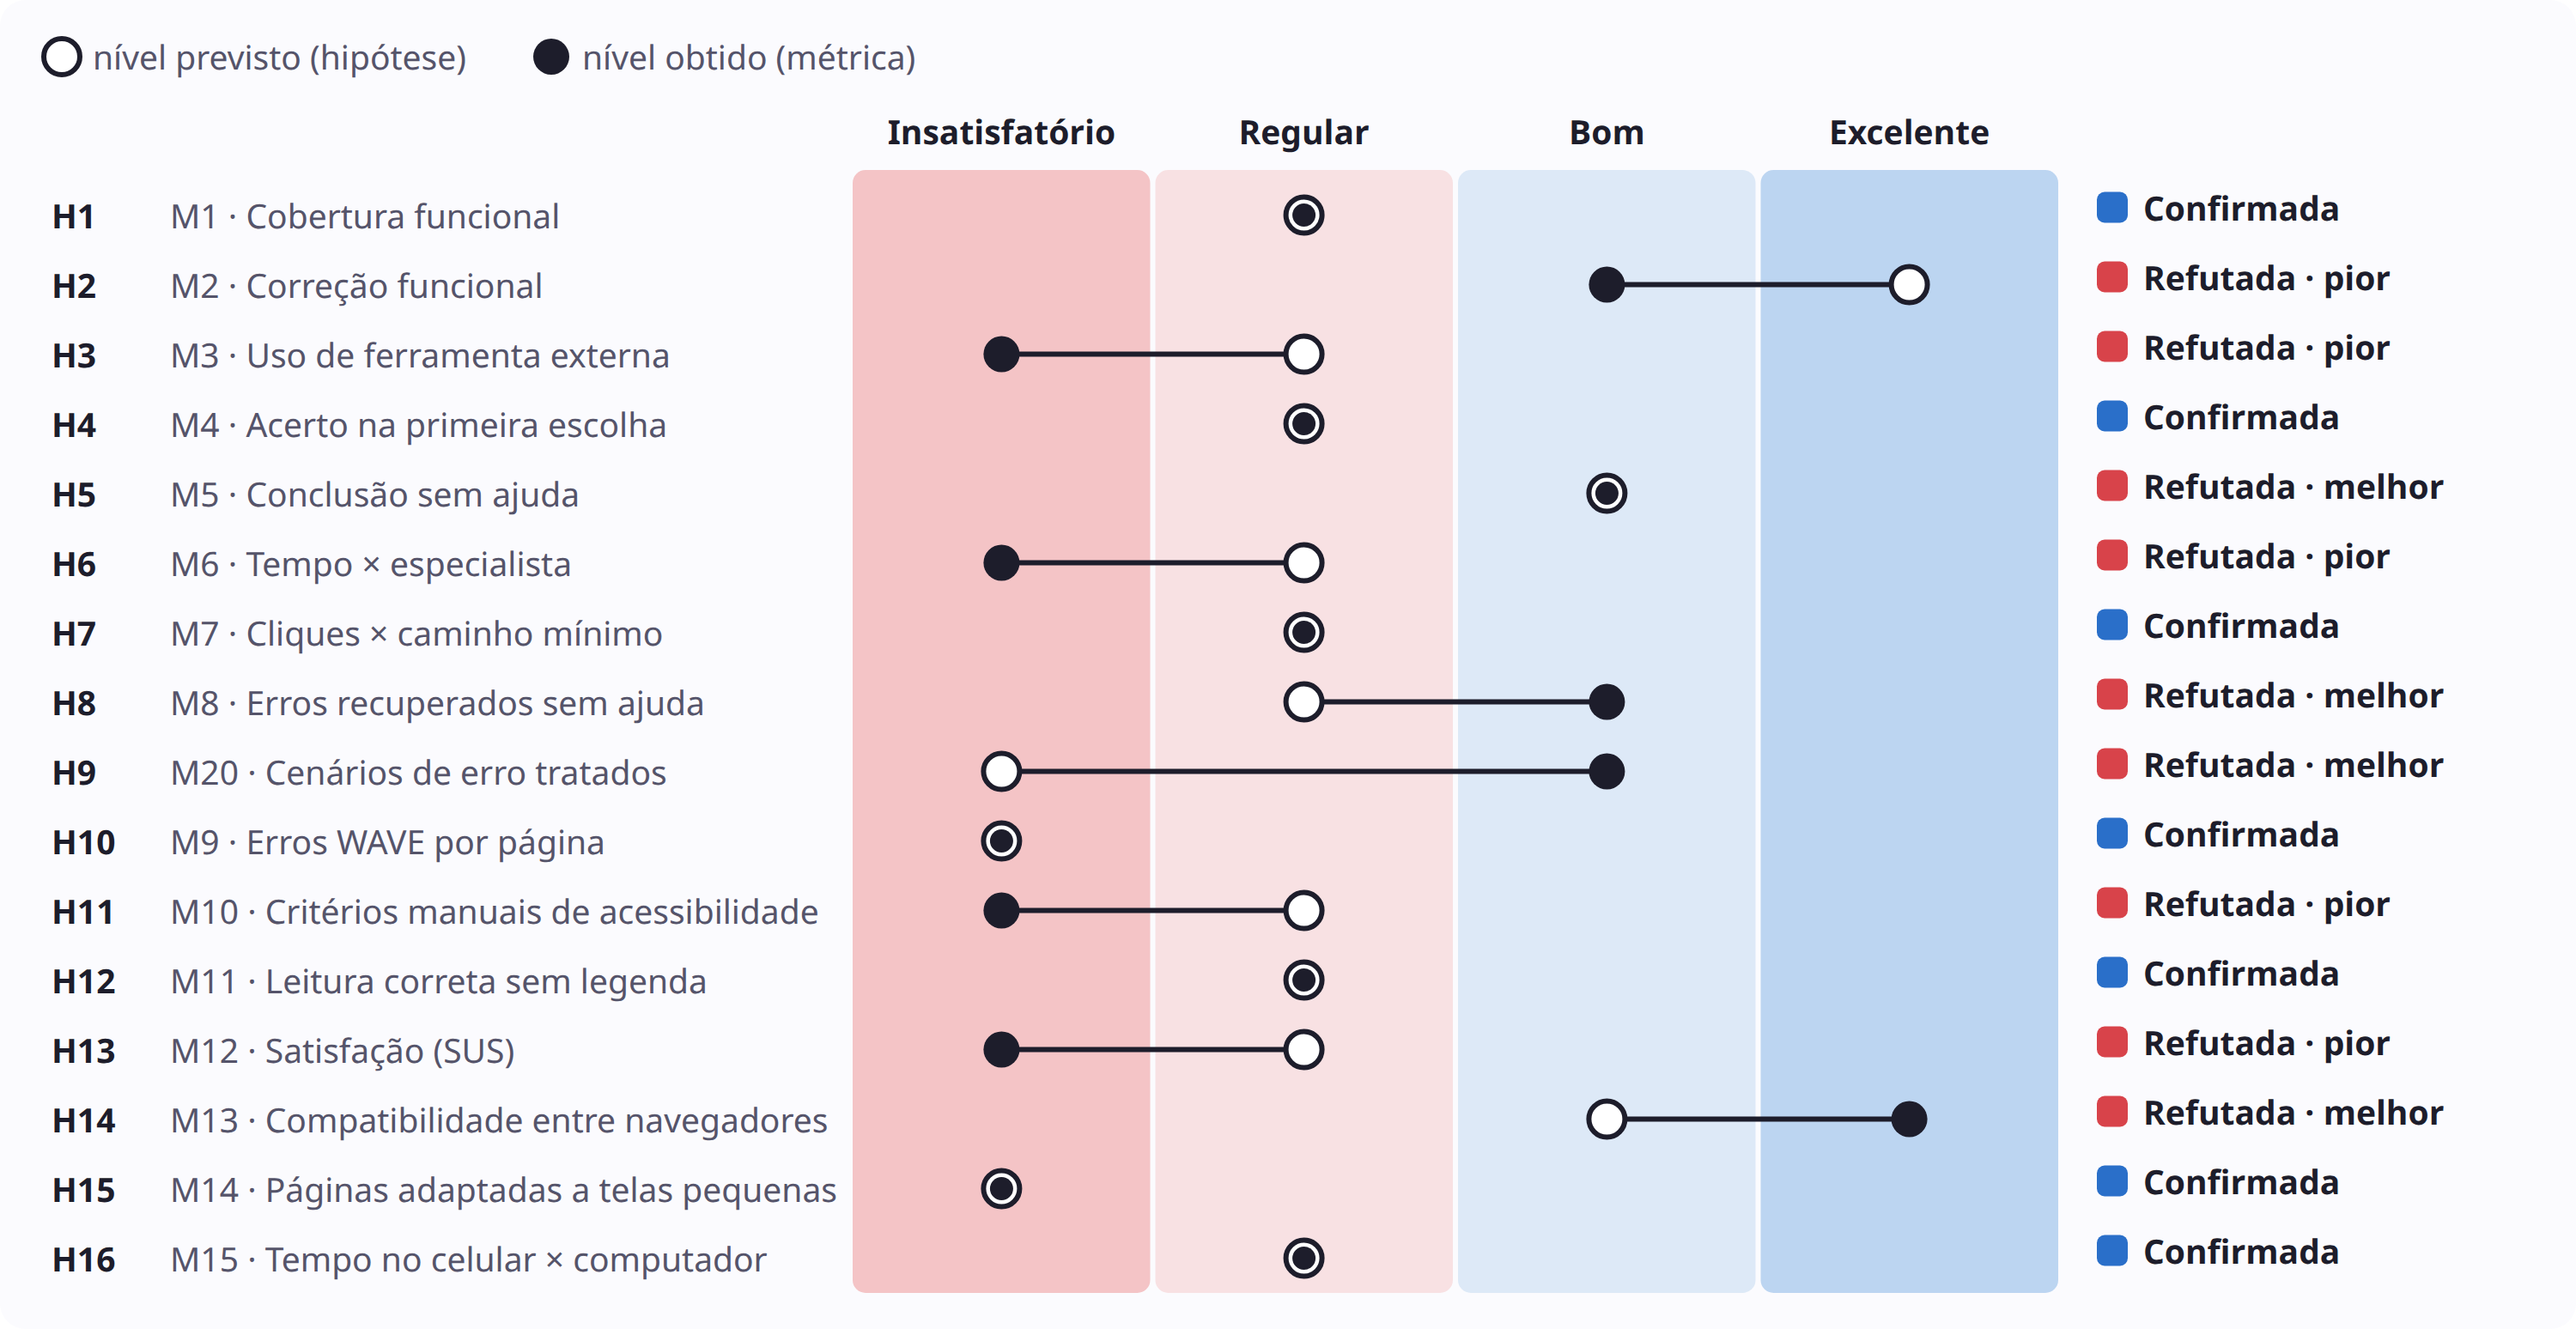
\includegraphics[width=0.8\textwidth]{figuras/hipoteses.png}
	\caption{Nível previsto por cada hipótese (círculo vazio) e nível obtido pela métrica (círculo cheio). Quando coincidem, a hipótese foi confirmada.}
	\label{fig:hipoteses}
	\fonte{elaborado pela equipe a partir de \texttt{dados/consolidados/metricas.csv} e das hipóteses da Fase 2.}
\end{figure*}

\textbf{Julgamento.} A Tabela~\ref{tab:julgamento} aplica as etapas 2 e 3 dos critérios de julgamento: a pontuação do objetivo é a média dos níveis das questões; a característica atende com média de pelo menos 2 e nenhuma questão Insatisfatória, e não atende com média abaixo de 1.

\begin{table}[!t]
	\caption{Julgamento das características}
	\label{tab:julgamento}
	\centering
	\footnotesize
	\setlength{\tabcolsep}{3pt}
	\begin{tabularx}{\columnwidth}{L{1.85cm} Y C{0.75cm} L{1.55cm}}
		\toprule
		\textbf{Característica} & \textbf{Níveis das questões} & \textbf{Média} & \textbf{Julgamento} \\
		\midrule
		Capacidade de Interação & Q4=1, Q5=2, Q6=0, Q7=1, Q8=2, Q9=2, Q10=0, Q11=0, Q12=1, Q13=0 & 0,90 & \textbf{Não atende} \\
		Adequação Funcional & Q1=1, Q2=2, Q3=0 & 1,00 & \textbf{Atende parcialmente} \\
		Flexibilidade & Q14=3, Q15=0, Q16=1 & 1,33 & \textbf{Atende parcialmente} \\
		\bottomrule
	\end{tabularx}
	\fonte{elaborado pela equipe.}
\end{table}

Em Flexibilidade, a média de 1,33 não descreve um sistema ``médio'': ela soma um ponto forte (Q14, Excelente) e um ponto crítico (Q15, Insatisfatório), e é a separação por questão que mostra onde está o problema. A relação HR1 (Flexibilidade $\rightarrow$ Capacidade de Interação) foi \textbf{estabelecida, com ressalva}: o celular exige 1,59 vez o tempo do computador, e as maiores razões estão em páginas não adaptadas; como nenhuma página é adaptada, não há como comparar com uma que seja. A relação HR2 (Capacidade de Interação $\rightarrow$ Adequação Funcional) \textbf{não foi estabelecida}: em nenhuma das 30 tentativas o participante afirmou que uma função existente não existia (MA1 = 0); quem não encontrou a função desistiu ou concluiu a tarefa fora do SIGAA.

\textbf{Ranking das tarefas.} Pela média dos níveis de M5, M6, M7 e M1 por tarefa, as piores são T6 (1,25) e T4 (1,33), as únicas com 60\% de conclusão sem ajuda. Em T6, três dos cinco participantes clicaram no link ``Calendário Acadêmico de Graduação'' do painel do portal, que abre a página de Pós-Graduação do site da SAA: um voltou ao SIGAA, um usou o calendário de fora (o que não conta como conclusão) e um desistiu. Em T4, a carga horária pendente está na página inicial, mas dois participantes desistiram, e os que a encontraram fizeram 5,67 cliques e levaram 8,48 vezes o tempo do especialista.

\subsection{Matriz multiplataforma (dado complementar)}
\label{sec:matriz}

M13 e M14 cobrem quatro navegadores de computador e duas larguras emuladas no Chrome. Para saber se o resultado de M14 depende do sistema, do aparelho ou do navegador, a equipe ampliou a execução instrumentada para uma matriz de \textbf{20 perfis}: dez de computador (Windows~11 com Chrome, Edge, Firefox, Opera e Brave; macOS com Safari e Chrome; Linux com Chromium, Chrome e Firefox), sete de celular (Android com Chrome em um Galaxy S24 e um Pixel~7, Edge em um Galaxy A55 e Opera em um Moto G4; iOS com Safari em três iPhones) e três de tablet (Galaxy Tab S9, iPad Mini e iPad Pro 11). Cada perfil usa o motor real do navegador (Blink, Gecko ou WebKit), com a largura, a densidade de pixels, o toque, o modo móvel e o \textit{user agent} do aparelho, tomados do catálogo de dispositivos do Playwright \cite{playwright}. Em cada perfil, o \textit{script} mediu a página de login da UnB, entrou no SIGAA, executou T1 a T6 e aplicou às páginas os critérios de M14, com a largura do aparelho no lugar de 360 e 768~px. A emulação não reproduz o sistema operacional em si (fontes, teclado virtual) nem o desempenho do aparelho; por isso, a matriz é dado complementar e não altera M13 nem M14.

\begin{figure*}[!t]
	\centering
	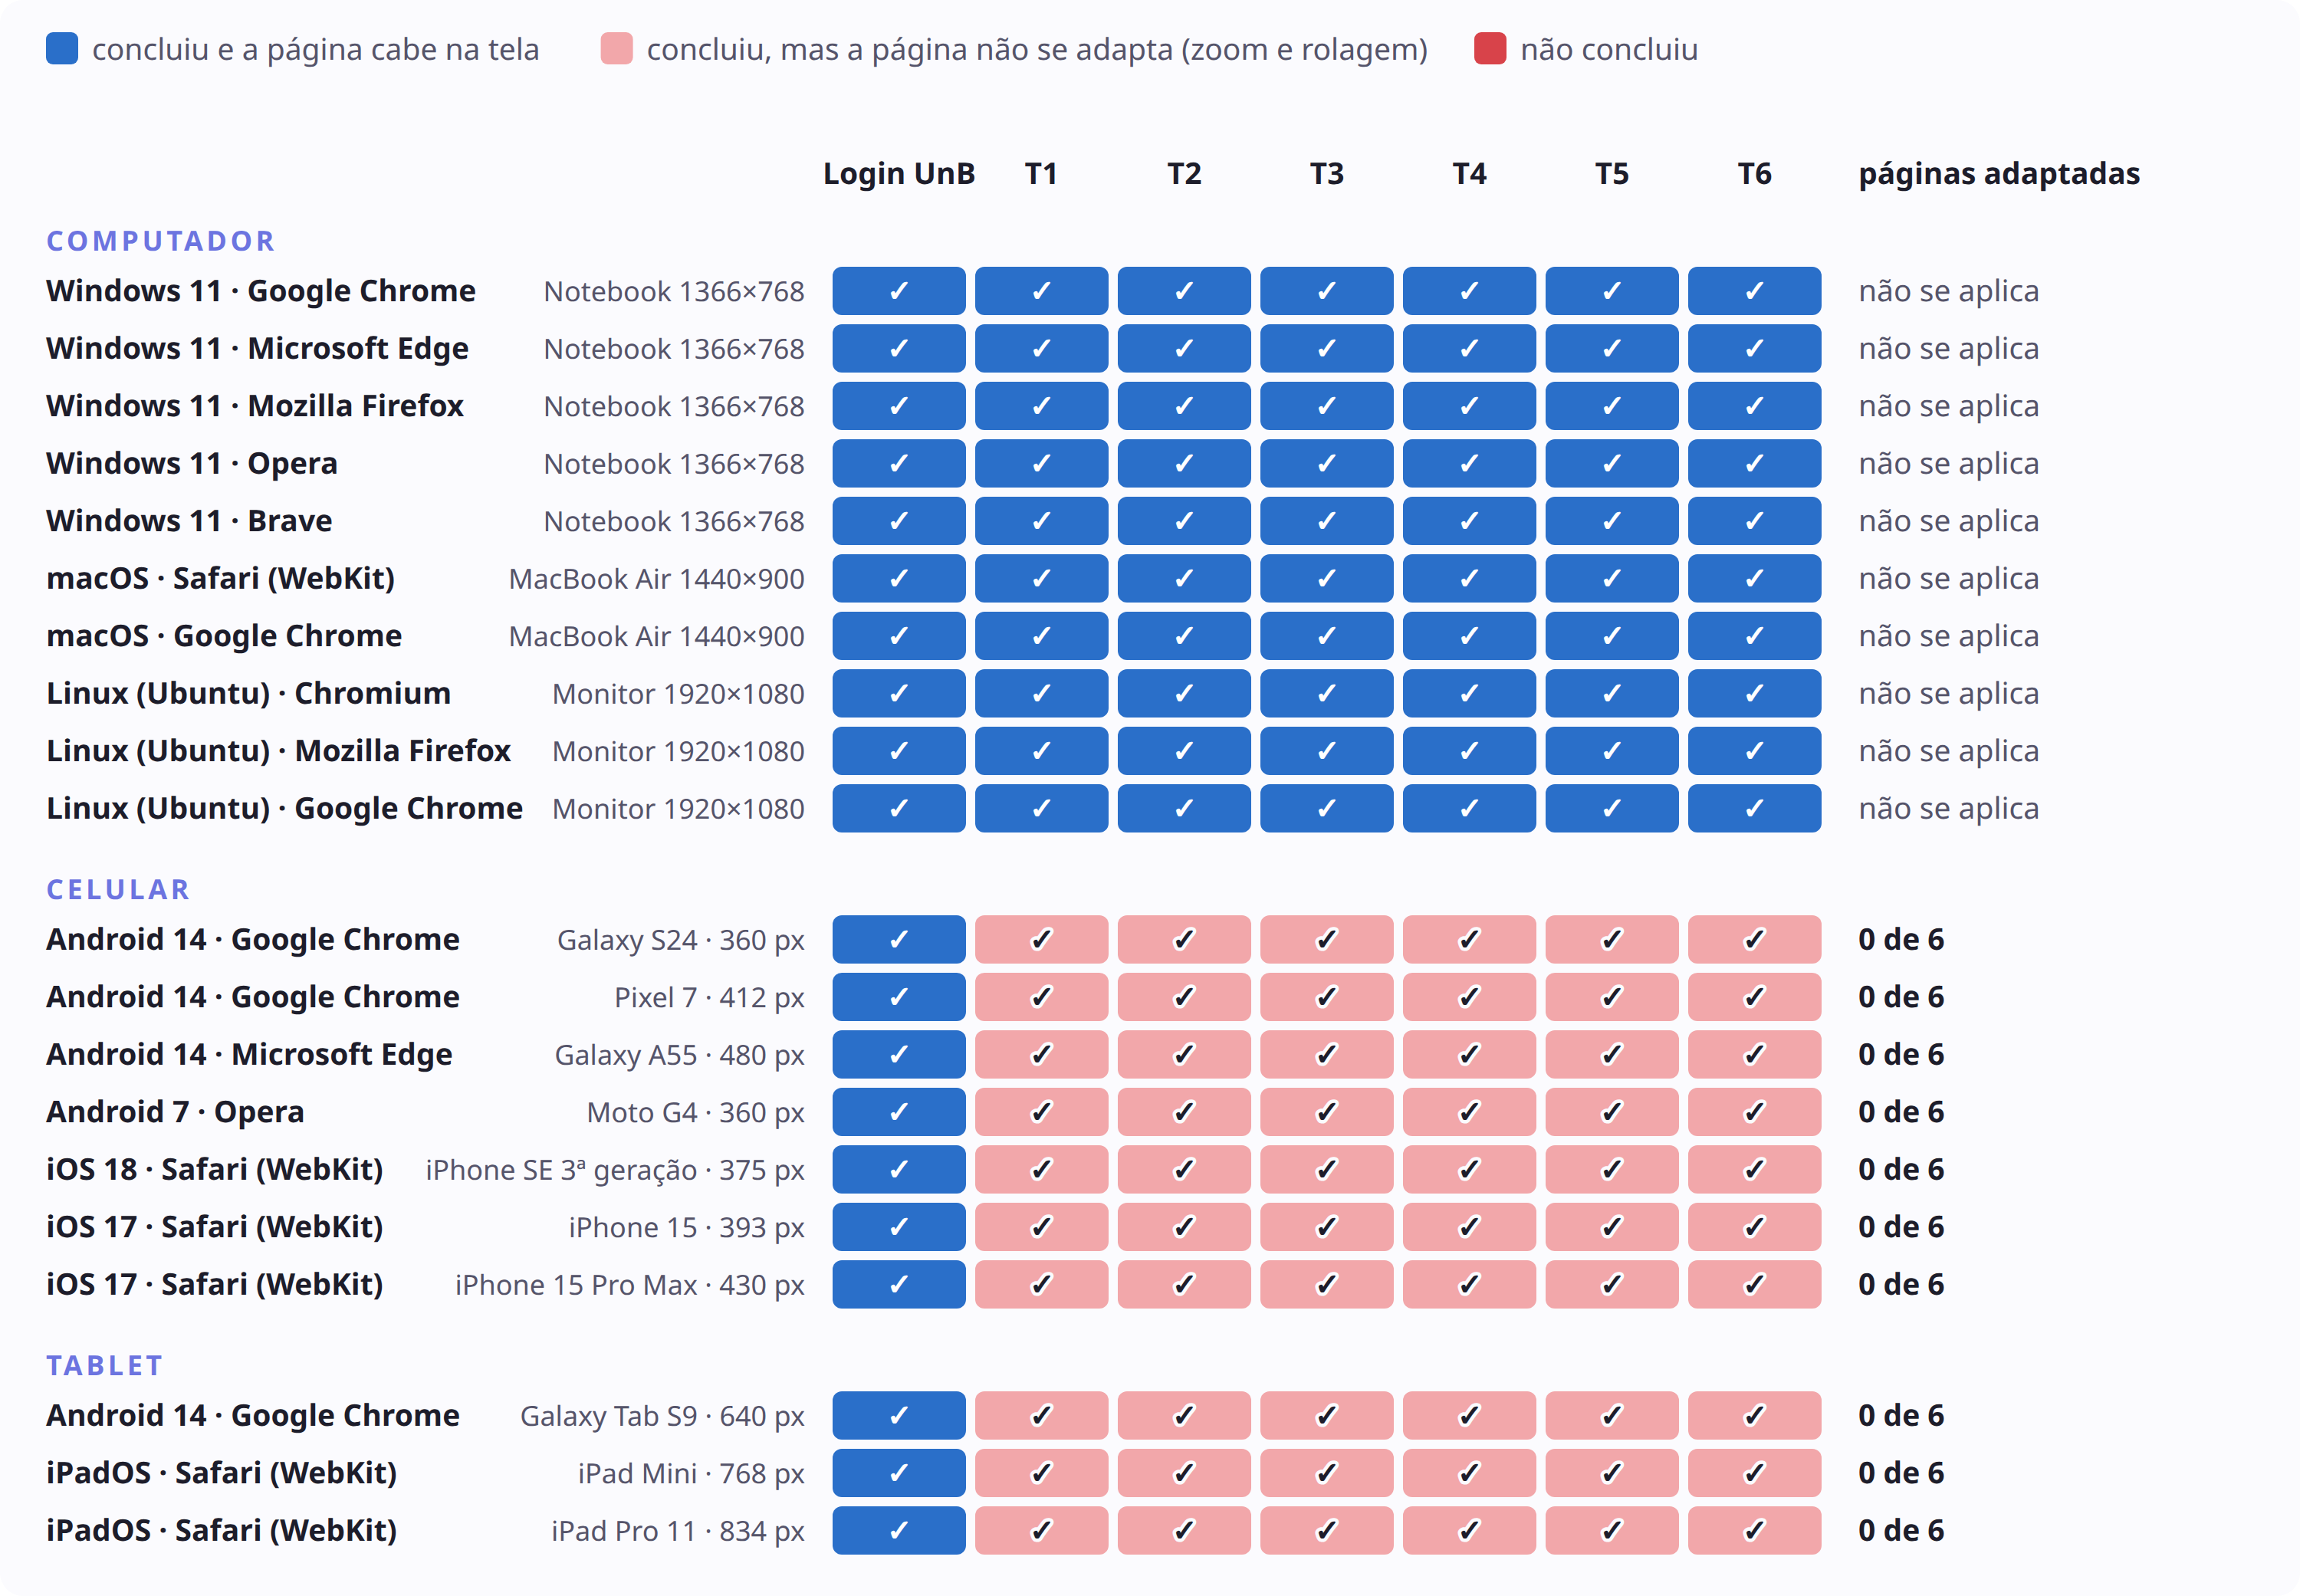
\includegraphics[width=0.84\textwidth]{figuras/matriz-multiplataforma.png}
	\caption{Matriz multiplataforma: página de login da UnB e tarefas T1 a T6 em 20 perfis de sistema, aparelho e navegador. Azul: concluiu e a página cabe na tela; rosa: concluiu, mas a página não se adapta.}
	\label{fig:matriz}
	\fonte{elaborado pela equipe a partir de \texttt{dados/consolidados/matriz-dispositivos.csv}.}
\end{figure*}

A coleta foi feita em 23/11/2026 (Fig.~\ref{fig:matriz}). As 120 execuções de tarefa terminaram com a página final correta, nos três motores, o que estende o resultado de M13 a Opera, Brave, Chromium, Safari no macOS e aos navegadores móveis. Nenhuma das 60 verificações de celular e tablet atendeu aos critérios de M14: o navegador mostra a página a 37\%--49\% da escala nos celulares e a 65\%--85\% nos tablets, e a menor fonte fica entre 2,9 e 3,9~px e entre 5,2 e 6,8~px, respectivamente. O resultado não depende do sistema, do navegador nem do tamanho da tela, de modo que M14 = 0\% não é efeito da emulação no Chrome. Em contraste, a página de login da UnB, no mesmo percurso, declara a \textit{viewport} e cabe na tela nos dez perfis móveis, com fonte mínima de 13 a 14~px; o único defeito, em quatro perfis, é o logotipo cobrir o texto de \textit{copyright} do rodapé. Os menus abriram ao toque nos 50 acionamentos; como a emulação toca o centro exato do alvo, o menu que não abriu para dois participantes é mais bem explicado pelo tamanho do item Ensino (cerca de 23~$\times$~9~px) do que pelo evento de toque. Dois achados de método: no WebKit em modo móvel, o toque do Playwright cai fora do alvo quando a página é reduzida, e o \textit{script} passou a corrigir a posição pela escala da área visível; e o Vivaldi não pôde ser automatizado. Mesmo no computador, a menor fonte do SIGAA é de 8~px em todos os perfis.

\subsection{Dados complementares de desempenho}
\label{sec:desempenho}

Os dados de Eficiência de Desempenho não têm questão nem nível, porque a característica saiu da especificação, mas foram coletados pelos mesmos \textit{scripts}, com o \textit{cache} desativado, em dois cenários: computador sem limitação de rede (cinco repetições) e celular de 360~px com a rede 4G e a CPU limitadas pelo perfil do Lighthouse \cite{lighthouse} (três repetições); 46 das 48 execuções foram válidas (Tabela~\ref{tab:desempenho}).

\begin{table}[!t]
	\caption{Espera pelo sistema e LCP (medianas)}
	\label{tab:desempenho}
	\centering
	\footnotesize
	\setlength{\tabcolsep}{2.5pt}
	\begin{tabularx}{\columnwidth}{L{0.45cm} C{0.95cm} C{0.95cm} C{1.0cm} Y C{1.0cm} C{0.9cm}}
		\toprule
		& \multicolumn{3}{c}{\textbf{Computador}} & \multicolumn{3}{c}{\textbf{Celular em 4G}} \\
		\cmidrule(lr){2-4}\cmidrule(lr){5-7}
		& \textbf{Espera (s)} & \textbf{TTFB (s)} & \textbf{LCP P75 (s)} & \textbf{Espera (s)} & \textbf{LCP P75 (s)} & \textbf{KB} \\
		\midrule
		T1 & 1,11 & 0,93 & 1,1 & 2,81 & 2,1 & 134 \\
		T2 & 1,03 & 0,35 & 1,2 & 8,55 & 7,0 & 567 \\
		T3 & 0,62 & 0,22 & 0,6 & 3,55 & 3,0 & 204 \\
		T4 & 1,62 & 0,98 & 1,7 & 6,51 & 5,4 & 504 \\
		T5 & 2,13 & 0,55 & 1,9 & 19,04 & 13,7 & 1955 \\
		T6 & 1,59 & 0,10 & 0,7 & 10,13 & 3,9 & 399 \\
		\bottomrule
	\end{tabularx}
	\fonte{elaborado pela equipe a partir de \texttt{dados/consolidados/desempenho.csv}. Espera: soma do carregamento das páginas da tarefa; KB: transferido na página final.}
\end{table}

No computador, fora do horário de pico, a espera ficou entre 0,62 e 2,13~s e o LCP no P75 abaixo de 1,9~s, na faixa ``boa'' dos Core Web Vitals \cite{webvitals}. Três pontos se destacam: o servidor responde devagar nas páginas que calculam dados do estudante (TTFB de 0,93~s nas notas e 0,98~s nos índices, acima do limite ``bom'' de 0,8~s); a Turma Virtual se desloca depois de pintada (CLS de 1,05, quatro vezes o limite ``ruim'' de 0,25); e, no celular em 4G, a espera passa dos 10~s em que o usuário perde a atenção \cite{nielsen1993} no calendário (10,1~s) e na Turma Virtual (19,0~s, com cerca de 1,9~MB). O estudante que depende do celular é penalizado duas vezes: pela tela, que nenhuma página adapta, e pela rede.
